\section{Durchführung}
\label{sec:Durchführung}
\begin{figure}[H]
  \centering
  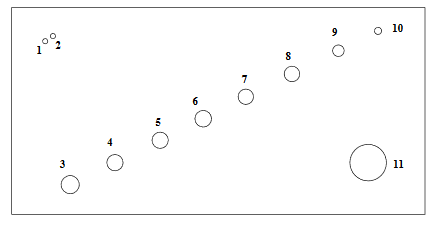
\includegraphics[height=5cm]{acryl.PNG}
  \caption{Abbildung des verwendeten Acrylblocks \cite{sample}.}
  \label{fig:acryl}
\end{figure}
Zu Beginn des Versuchs wird ein zu untersuchender Acryl-Block (zu erkennen in Abbildung \ref{fig:acryl})
von Hand mit einer Schieblehre vermessen. Dabei werden jeweils seine Kantenlängen sowie auch die
Abstände der einzelnen Fehlstellen zum oberen bzw. unteren Rand gemessen. Mit Abstand ist dabei die
senkrechte Strecke vom Rand des Blocks bis zum entsprechend äußersten Punkt der Fehlstelle gemeint.

Anschließend wird der Acryl-Block dann mit einem Ultraschallechoskop untersucht. Dieses ist an
einen Computer angeschlossen, welcher die gemessenen Daten graphisch darstelllt.
Mit einer an das Echoskop angeschlossenen Ultraschallsonde gibt man einen Ultraschallimpuls
in den Acrylblock. Als Koppelmittel wird dabei destilliertes Wasser verwendet. Die Sonde
kann ebenfalls eintreffende Impulse messen, sodass sie die von den Fehlstellen reflektierten
Impulse wahrnimmt.

Zu Beginn wird ein sogennanter A-Scan durchgeführt. Dabei lässt man den Computer die gemessenen
reflektierten Ultraschallimpulse in Abhängigkeit von der Zeit auf dem Bildschirm ausgeben.
Daraus wird für die einzelnen Löcher jeweils die Zeit bestimmt, nach welcher der an ihnen
reflektierte Impuls wieder an der Sonde eintrifft. Die Sonde muss also immer an den entsprechenden senkrechten
Punkt des Randes zur Fehlstelle geschoben werden. Dies wird einmal von der Oberseite und einmal
von der Unterseite des Acrylblocks durchgeführt.

Anschließend wird dann ein B-Scan durchgeführt. Dieser funktioniert ganz ähnlich, jedoch misst man
dabei nicht jede Fehlstelle einzeln aus, sondern schiebt die Sonde nur ein einziges mal oben bzw. auch wieder
unter über den Block. Der Rechner gibt dann in Abhängigkeit von der Zeit und der Tiefe den gemessenen
Impuls aus. Aus dieser Graphik wird dann direkt für alle Fehlstellen die Tiefe abgelesen.

Als letztes wird dann noch ein Herzmodell untersucht.
Dafür wird dieses zu einem drittel mit Wasser gefüllt. Sodann befestigt man eine Ultraschallsonde
über der Wasseroberfläche, sodass diese das Wasser nur leicht berührt. Mit einem A-Scan misst man den
von der Unterseite des Modells reflektierten Ultraschallimpuls. Danach wird das Herzvolumen mit einem
zu Verfügung stehenden Gummiball geändert, indem man mit diesem Luft in das Modell pumpt, welche eine bewegliche
Membran von unten in das Wasser drückt. Dann wird erneut ein A-Scan durchgeführt.
Anschließend wird dann ein TM-Scan gemacht. Bei diesem trägt der Rechner den gemessenen Impuls gegen die Zeit auf.
Bei der Messung wird 20 mal mit dem Gummiball Luft in das Modell gepumpt und wieder abgelassen. Aus der entstehenden
Graphik wird die Frequenz der sich ändernden Impulse sowie deren Amplitude bestimmt.
